\documentclass{article}
\newcommand\tab[1][1cm]{\hspace*{#1}}
\usepackage{fancyhdr}
\usepackage{enumerate}
\usepackage{amsmath}
\usepackage{amsfonts}
\usepackage{amssymb}
\usepackage{tikz}
\usetikzlibrary{arrows,automata}
\usepackage{graphicx}
\usepackage{grffile}

%
% Basic Document Settings
%

\topmargin=-0.45in
\evensidemargin=0in
\oddsidemargin=0in
\textwidth=6.5in
\textheight=9.0in
\headsep=0.25in

\linespread{1.1}

\pagestyle{fancy}
\lhead{\hmwkAuthorName}
\rhead{\hmwkClass: \hmwkTitle}
\cfoot{\thepage}

\renewcommand\headrulewidth{0.4pt}
\renewcommand\footrulewidth{0.4pt}

\setlength\parindent{0pt}

%
% Homework Details
%   - Title
%   - Due date
%   - Class
%   - Section/Time
%   - Instructor
%   - Author
%

\newcommand{\hmwkTitle}{Homework\ \#5}
\newcommand{\hmwkDueDate}{April 26, 2017}
\newcommand{\hmwkClass}{CS 344}
\newcommand{\hmwkClassTime}{Section \#1}
\newcommand{\hmwkClassInstructor}{Professor Bahman Kalantari}
\newcommand{\hmwkAuthorName}{\textbf{Douglas Rudolph, Mustufa Hussain}}

%
% Title Page
%

\title{
    \vspace{2in}
    \textmd{\textbf{\hmwkClass:\ \hmwkTitle}}\\
    \normalsize\vspace{0.1in}\small{Due\ on\ \hmwkDueDate\ at 11:59pm}\\
    \vspace{0.1in}\large{\textit{\hmwkClassInstructor\ \hmwkClassTime}}
    \vspace{3in}
}

\author{\hmwkAuthorName}
\date{}

\setlength\parskip{\baselineskip}

\begin{document}

\maketitle

\pagebreak

\section*{Problem 1: Use the fact that 3-CNF is NP-complete to prove NP-completeness of testing if a linear system of inequalities $Ax \leq b$ has a solution, where A is an $m \times n$ matrix of integer coefficients, x is a vector with n components consisting of either 0 or 1, and b is a vector with m integer components. Here $Ax \leq b$ means the inequality must be satisfied component-wise.}
To show that this is the case, we have to show i) that the above problem is in NP ii) that 3-CNF can be reduced in polynomial time to the above problem. \\
Proof of i): To show that the above is NP, it suffices to provide a polynomial time algorithm that, given a solution with a certificate of verification, checks that the provided solution is valid. This can be accomplished in two steps: 
\begin{enumerate}
\item Plug in the solution vector $s$ into $Ax \leq b$
\item For each of the m constraints, verify that the inequality is satisfied
\end{enumerate}
Clearly, this algorithm runs in polynomial time ($O(mn)$ to plug in the solution vector and $O(m)$ to check each constraint $\implies O(mn)$ algorithm) as desired.  \\
Proof of ii): To prove this, we must describe how to convert a general 3-CNF problem into the form $Ax \leq b$. Given a 3-CNF of the form $(x \vee y  \vee z) \wedge \dots \wedge (a \vee b \vee c)$ where x,y,z,a,b, and c are boolean variables, we know that the expression will evaluate to true if each individual clause evaluates to true. In the case of our linear system, this is equivalent to having each constraint hold true. As such, we can think of each clause in 3-CNF as a linear constraint. Additionally, we know that a given 3-CNF clause will evaluate to true if at least one variable in the clause is true. If we represent true with 1 and 0 with false, this is equivalent to asking if the sum of the variables is greater than 1. This leads to a formula that models a clause a constraint: Asking if $(x \vee y  \vee z)$ evaluates to true is equivalent to asking $x + y + z \geq 1$. It is also worth mentioning that if a given variable is a complement (i.e. of the form $\overline{x}$, we can represent it as $1-x$ in our constraint (i.e. if it is false, it adds one to the boolean sum while it adds nothing if it is true). Finally, to make the inequalities of the form $Ax \leq b$, we can simply negate both sides of each constraint to convert each $\geq$ into a $\leq$. This gives us a linear system of the form $Ax \leq b$ where A is our $m \times n$ constraint matrix, where each row corresponds to a 3-CNF clause, $x$ is a vector with n components, each of which is 0 or 1, and b is our vector of m constraints where each component is -1. Given n 3-CNF clauses, we can reduce it to the equivalent linear system with approximately 3*n operations, which corresponds to a polynomial time algorithm ($O(n)$) as desired. 

\section*{Problem 2: Consider the CNF expression $(x_1 \vee \overline{x_2} \vee x_3) \wedge (\overline{x_1} \vee x_2 \vee x_3) \wedge (x_1 \vee \overline{x_3}) \wedge (x_2 \vee \overline{x_3} \vee x_4)$. Convert this CNF into a graph so that G has a clique of size 4 iff the CNF is satisfiable. Does G have a clique of size 4?}
To convert the above CNF expression into a graph, we create a vertex for each literal and put an edge between vertices that don't belong to the same clause or contradict each other: \\

\begin{center}
		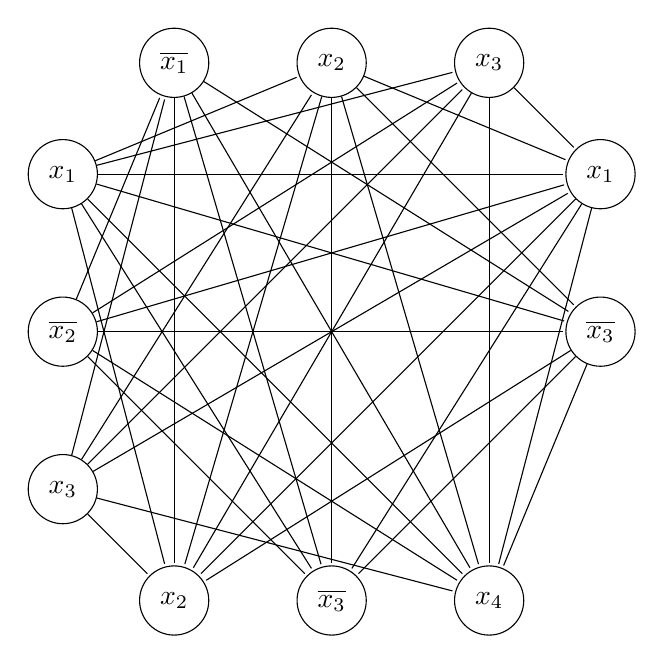
\begin{tikzpicture}[>=stealth',shorten >=1pt,auto,node distance=2cm]
        	\node[state]  (x11)  []           {$x_1$};
  			\node[state]   (xb21) [below of=x11]  {$\overline{x_2}$};
           \node[state]   (x31) [below of=xb21]  {$x_3$};
           
           
           \node[state]   (xb12) [above right of=x11]  {$\overline{x_1}$};
		   \node[state]   (x22) [right of=xb12]  {$x_2$};
           \node[state]   (x32) [right of=x22]  {$x_3$};
           
           \node[state]  (x13)  [below right of=x32]           {$x_1$};
            \node[state]  (xb33)  [below of=x13]           {$\overline{x_3}$};
            
            
            \node[state] (x24) [below right of=x31] {$x_2$};
            \node[state] (xb34) [right of=x24] {$\overline{x_3}$};
            \node[state] (x44) [right of=xb34] {$x_4$};
  			\path[] 
                     (x11) edge (x22)
                     (x11) edge (x32)
                     (x11) edge (x13)
                     (x11) edge (xb33)
                     (x11) edge (x44)
                     (x11) edge (xb34)
                     (x11) edge (x24)
                     
                     (xb21) edge (xb12)
                     (xb21) edge (x32)
                     (xb21) edge (x13)
                     (xb21) edge (xb33)
                     (xb21) edge (x44)
                     (xb21) edge (xb34)
                     
                     (x31) edge (xb12)
                     (x31) edge (x22)
                     (x31) edge (x32)
                     (x31) edge (x13)
                     (x31) edge (x44)
                     (x31) edge (x24)
                     
                     (xb12) edge (xb33)
                     (xb12) edge (x44)
                     (xb12) edge (xb34)
                     (xb12) edge (x24)
                     
                     (x22) edge (x13)
                     (x22) edge (xb33)
                     (x22) edge (x44)
                     (x22) edge (xb34)
                     (x22) edge (x24)
                     
                     (x32) edge (x13)
                     (x32) edge (x44)
                     (x32) edge (x24)
                     
                     (x13) edge (x44)
                     (x13) edge (xb34)
                     (x13) edge (x24)
                     
                     (xb33) edge (x44)
                     (xb33) edge (xb34)
                     (xb33) edge (x24)
                     ;
        	         
            	 		
		\end{tikzpicture}
	\end{center}

The graph does indeed have a clique of size 4 (given by setting $x_1$ and $x_2$ to true in the CNF problem); the nodes that form the clique are double circled and the edges which form the clique are included (all others are omitted for readability):

\begin{center}
		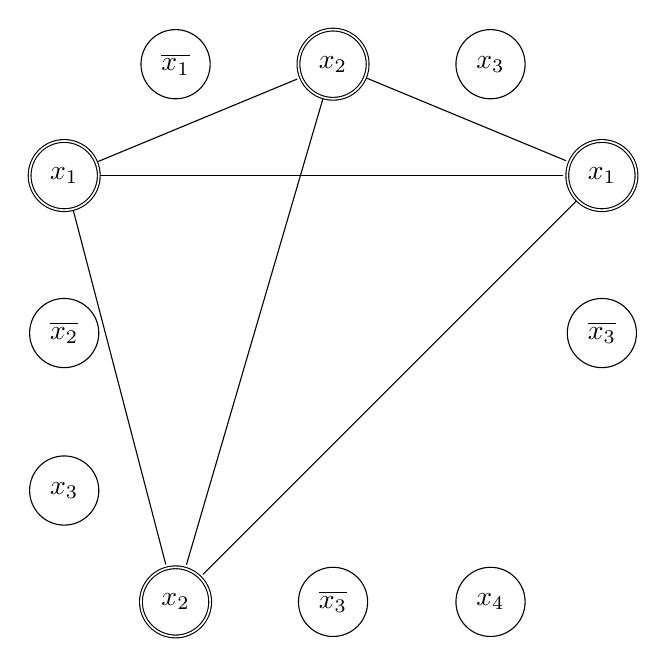
\begin{tikzpicture}[>=stealth',shorten >=1pt,auto,node distance=2cm]
        	\node[state, accepting]  (x11)  []           {$x_1$};
  			\node[state]   (xb21) [below of=x11]  {$\overline{x_2}$};
           \node[state]   (x31) [below of=xb21]  {$x_3$};
           
           
           \node[state]   (xb12) [above right of=x11]  {$\overline{x_1}$};
		   \node[state, accepting]   (x22) [right of=xb12]  {$x_2$};
           \node[state]   (x32) [right of=x22]  {$x_3$};
           
           \node[state, accepting]  (x13)  [below right of=x32]           {$x_1$};
            \node[state]  (xb33)  [below of=x13]           {$\overline{x_3}$};
            
            
            \node[state, accepting] (x24) [below right of=x31] {$x_2$};
            \node[state] (xb34) [right of=x24] {$\overline{x_3}$};
            \node[state] (x44) [right of=xb34] {$x_4$};
  			\path[] 
                     (x11) edge (x22)
                     (x11) edge (x13)
                     (x11) edge (x24)
                     
                     (x22) edge (x13)
                     (x22) edge (x24)
                     
                     (x13) edge (x24);
             \end{tikzpicture}
	\end{center}
\pagebreak
\section*{Problem 3: For the graph G = (V, E) above construct the complement graph $\overline{G} =
(V, \overline{E})$. What is the largest clique in G? what is the largest vertex-cover in $\overline{G}$?}
We construct the complement graph, $\overline{G}$:
\begin{center}
		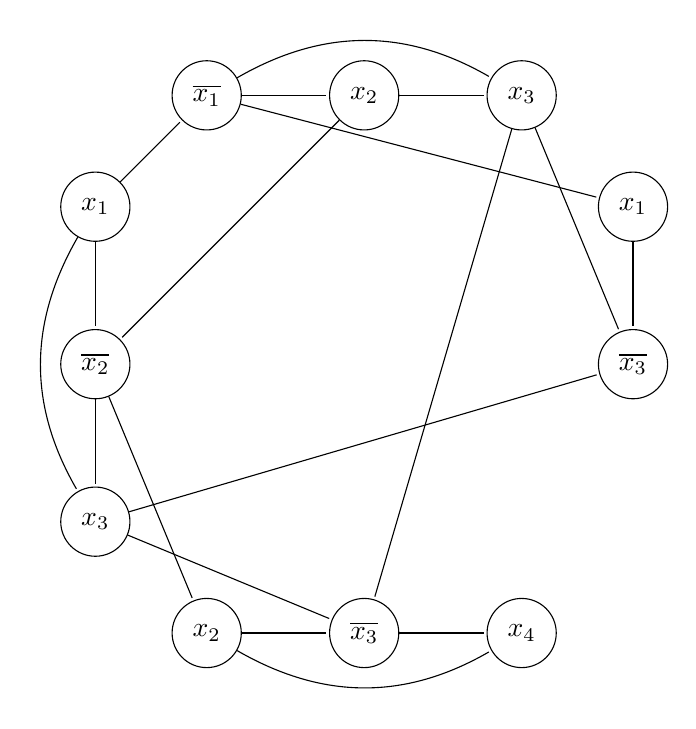
\begin{tikzpicture}[>=stealth',shorten >=1pt,auto,node distance=2cm]
        	\node[state]  (x11)  []           {$x_1$};
  			\node[state]   (xb21) [below of=x11]  {$\overline{x_2}$};
           \node[state]   (x31) [below of=xb21]  {$x_3$};
           
           
           \node[state]   (xb12) [above right of=x11]  {$\overline{x_1}$};
		   \node[state]   (x22) [right of=xb12]  {$x_2$};
           \node[state]   (x32) [right of=x22]  {$x_3$};
           
           \node[state]  (x13)  [below right of=x32]           {$x_1$};
            \node[state]  (xb33)  [below of=x13]           {$\overline{x_3}$};
            
            
            \node[state] (x24) [below right of=x31] {$x_2$};
            \node[state] (xb34) [right of=x24] {$\overline{x_3}$};
            \node[state] (x44) [right of=xb34] {$x_4$};
  			\path[] 
                     (x11) edge (xb21)
                     (xb21) edge (x31)
                     (x11) edge [bend right] (x31)
                     (x11) edge (xb12)
                     
                     (xb12) edge (x22)
                     (x22) edge (x32)
                     (xb12) edge [bend left] (x32)
                     (xb12) edge (x13)
                     (x22) edge (xb21)
                     
                     (x13) edge (xb33)
                     (x32) edge (xb33)
                     (x31) edge (xb33)
                     (x32) edge (xb34)
                     (xb21) edge (x24)
                     (x31) edge (xb34)
                     (x24) edge [bend right] (x44)
                     (x24) edge (xb34)
                     (xb34) edge (x44)
                     ;
             \end{tikzpicture}
	\end{center}
    
    The largest clique in G is equivalent to the maximum size of sets of nonadjacent vertices in $\overline{G}$. These sets are as follows: 
\begin{enumerate}
\item $\{x_1, x_4, x_2, x_3\}$
\item $\{\overline{x_3}, x_4, \overline{x_2}, \overline{x_1}\}$
\item $\{x_2, x_3, x_2, x_1\}$
\item $\{\overline{x_3}, \overline{x_2}, \overline{x_1}, \overline{x_3}\}$
\item $\{x_4, x_3, x_2, x_1\}$
\item $\{x_3, x_2, x_1, x_4\}$
\end{enumerate}

As such, we conclude that the largest clique size is 4. \\

Because our largest clique is of size 4 and there are 11 vertices, we know that our vertex cover will be of size 7 (vertices in the vertex denoted by double circles):  

\begin{center}
		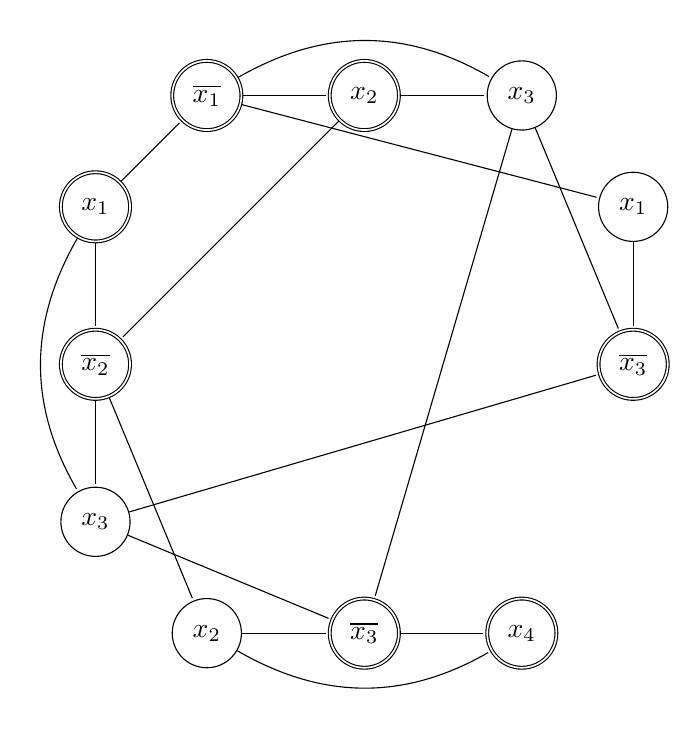
\begin{tikzpicture}[>=stealth',shorten >=1pt,auto,node distance=2cm]
        	\node[state, accepting]  (x11)  []           {$x_1$};
  			\node[state, accepting]   (xb21) [below of=x11]  {$\overline{x_2}$};
           \node[state]   (x31) [below of=xb21]  {$x_3$};
           
           
           \node[state, accepting]   (xb12) [above right of=x11]  {$\overline{x_1}$};
		   \node[state, accepting]   (x22) [right of=xb12]  {$x_2$};
           \node[state]   (x32) [right of=x22]  {$x_3$};
           
           \node[state]  (x13)  [below right of=x32]           {$x_1$};
            \node[state, accepting]  (xb33)  [below of=x13]           {$\overline{x_3}$};
            
            
            \node[state] (x24) [below right of=x31] {$x_2$};
            \node[state, accepting] (xb34) [right of=x24] {$\overline{x_3}$};
            \node[state, accepting] (x44) [right of=xb34] {$x_4$};
  			\path[] 
                     (x11) edge (xb21)
                     (xb21) edge (x31)
                     (x11) edge [bend right] (x31)
                     (x11) edge (xb12)
                     
                     (xb12) edge (x22)
                     (x22) edge (x32)
                     (xb12) edge [bend left] (x32)
                     (xb12) edge (x13)
                     (x22) edge (xb21)
                     
                     (x13) edge (xb33)
                     (x32) edge (xb33)
                     (x31) edge (xb33)
                     (x32) edge (xb34)
                     (xb21) edge (x24)
                     (x31) edge (xb34)
                     (x24) edge [bend right] (x44)
                     (x24) edge (xb34)
                     (xb34) edge (x44)
                     ;
             \end{tikzpicture}
	\end{center}
We can find the above by starting with one of our sets (say $\{\overline{x_3}, \overline{x_2}, \overline{x_1}, \overline{x_3}\}$) and denoting adjacent edges. After this, we pick the vertices with leftover edges, namely $\{x_1, x_2, x_4\}$, giving us our vertex cover.

\section*{Problem 4: Suppose $G = (V, E)$ is a spanning tree. Describe an algorithm that would
efficiently compute a minimum vertex-cover for G}

Given an undirected graph $G$, we know that a spanning tree of the graph $G$ is a subgraph that is made up of a collection of edges that connects all the verticies together. Because we know that this subgraph is made up of a collection of edges that manage to connect every vertex within the graph, then we know that the spanning tree is a filtered subset of the verticies that are apart a vertex cover. 

In order to find the vertex cover, we can simply start by looking at the node with the highest degree within the spanning tree. Now that we have the node with the highest degree, we can mark that node as inside the vertex cover, and remove said node and all neighboring nodes from the set of verticies that are within the spanning tree. This process can then be repeated on the next node with the highest degree until there are no longer no more nodes within the set of the subgraph. The remainng marked nodes is the considered to be the vertex cover. 
\end{document}